\section{Methodology}

\lettrine{T}{he} prospective solution was ultimately named \emph{Packet Courier} for reasons that the ensuing design
documentation aims to make clear. In summary, Packet Courier listens for packets being sent by nodes on its virtual
network, processing and rerouting them according to their listed destination and the associated conditions; just as a
mail courier would do analogously for letters and parcels. The metaphor also aligns itself well with the overall
motivations of the project, whereby postal services are largely seen as reliable infrastructure that operate silently
in the background, enabling people to send goods across seemingly vast distances without needing to worry about how
this is achieved. Indeed, these are the ideals that Packet Courier strives to embody, especially in light of
objectives 4) and 5).

Packet Courier has been designed and developed by leveraging philosophies from the \emph{lean development} school of
thought\cite{william_feld_lean_book, steve_blank_lean_blog}. This involved making Packet Courier a functional and
useful piece of software from the very first iteration, and continuing to ensure that this remained so with each new
feature. As a consequence, every supervisory meeting, informal peer review or user ``playtest'' would be a
meaningfully different experience, with something novel to demonstrate on each occasion. In this way, any feedback
could be readily taken on-board and implemented quickly. By contrast, if Packet Courier had been meticulously
designed from the bottom-up or the top-down, even the smallest changes in direction could risk rendering much of the
planning totally obsolete.

The simplest way to guarantee that Packet Courier provided users with tangible value from day one was to integrate an
application-programmer interface into the base simulation engine. That way, developers could always take advantage of
what Packet Courier had to offer, even if it was primitive. This ended up paying dividends down-the-line, as it was this
combination of design philosophy and system architecture that facilitated the development of Packet Courier's
emulation mode, which leveraged the base simulation APIs to further empower Packet Courier to manipulate authentic
UDP packets in real-time.


\section{High-Level Architecture}

\subsection{Simulation Semantics}

\lettrine{M}{any} of Packet Courier's core abstractions are inspired by the Elixir programming language\cite{elixir}.
One of Elixir's major selling points is how elegantly it removes unnecessary detail when interfacing with the
programmer. Rather than hemming developers into considering bits being sent over a wire, or packets being sent over a
network, Elixir talks in terms of \emph{processes} exchanging \emph{messages} with one
another\cite{elixir_processes}, which could consist of any high-level object such as text, numbers, tuples, or even
higher-order structures like lists and structs. Furthermore, Elixir uses neat allegories to help developers build up
a more intuitive picture of what their code does, i.e.: collecting messages from a \emph{mailbox} or using an
arbitrary \emph{process-id} rather than an ip-address. Not only does this improve readability, but it also insulates
the logic of the distributed algorithms from the lower-level details of the machine or the network. Is \texttt{ipv4}
or \texttt{ipv6} being used? An Elixir developer wouldn't need to know or care.

As such, Packet Courier channels Elixir's spirit of using intuitive, high-level concepts to help users quickly build
an understanding for a given simulation. As one might expect, the \emph{Node} is a cornerstone abstraction within the
Packet Courier framework. A node represents a particular location within a wider network topology and enjoys a unique
\emph{Node Address}. Each node will have at least one \emph{Worker}, where each worker will in turn carry out some
work in the form of a coroutine. Workers also have access to a \emph{Postal Service} which enables them to interact
with the wider network by sending a \emph{Packet} to a destination \emph{WorkerAddress}. The postal service will then
package the packet and destination worker address into a single piece of \emph{Mail} and send it along the
\emph{Node Connection} associated with the source and destination worker addresses (provided it exists). Notice that
the mail is sent along a node connection, as opposed to a \emph{worker} connection, because mail is principally
exchanged between nodes rather than workers. In this way, when a piece of mail arrives at its destination node, the
node extracts and routes the packet to its respective worker address; idiomatically speaking, the node
\emph{Delivers} the packet to the worker's \emph{Mailbox}. The worker then has the option to poll packets from its
mailbox. It is important to note that mailboxes store packets, not \emph{mail}. The rationale behind this is that one
needn't accompany their letter or parcel with a return address in order to send it; this is a choice that can be made
at the sender's discretion. Workers are also granted privacy, meaning that they can only see the contents of their own
mailbox.

Drilling down into the specifics of packet transmission, each node connection is associated with a \emph{Packet
Pipeline}. As the name suggests, a packet pipeline is a linear conduit whereby packets are processed in a fashion
akin to a conveyor-belt, and it is herein that any packet manipulation is conducted, i.e.: latency, drop, corruption.
The nature of this architecture is the first reason why packet communication occurs between nodes and not workers. If
$n$ nodes had on average $w$ workers each, then the maximum number of unidirectional inter-node connections would be
$n(n-1)$, yet the expected number of unidirectional inter-worker connections would be $w^2n(n-1)$. Thus, it is much
more resource efficient for the workers to simply delegate mail sorting responsibilities to their respective node. In
addition, workers are temporal insofar as they can be added and removed from the simulation dynamically like threads,
which would mean that packet pipelines would need to be introduced on-the-fly in a way that would only mirror
node-to-node semantics anyway, since workers inherit their position in the topology (i.e.: who they can send packets
to and with what network conditions) from their node.

\begin{figure}[!h]
    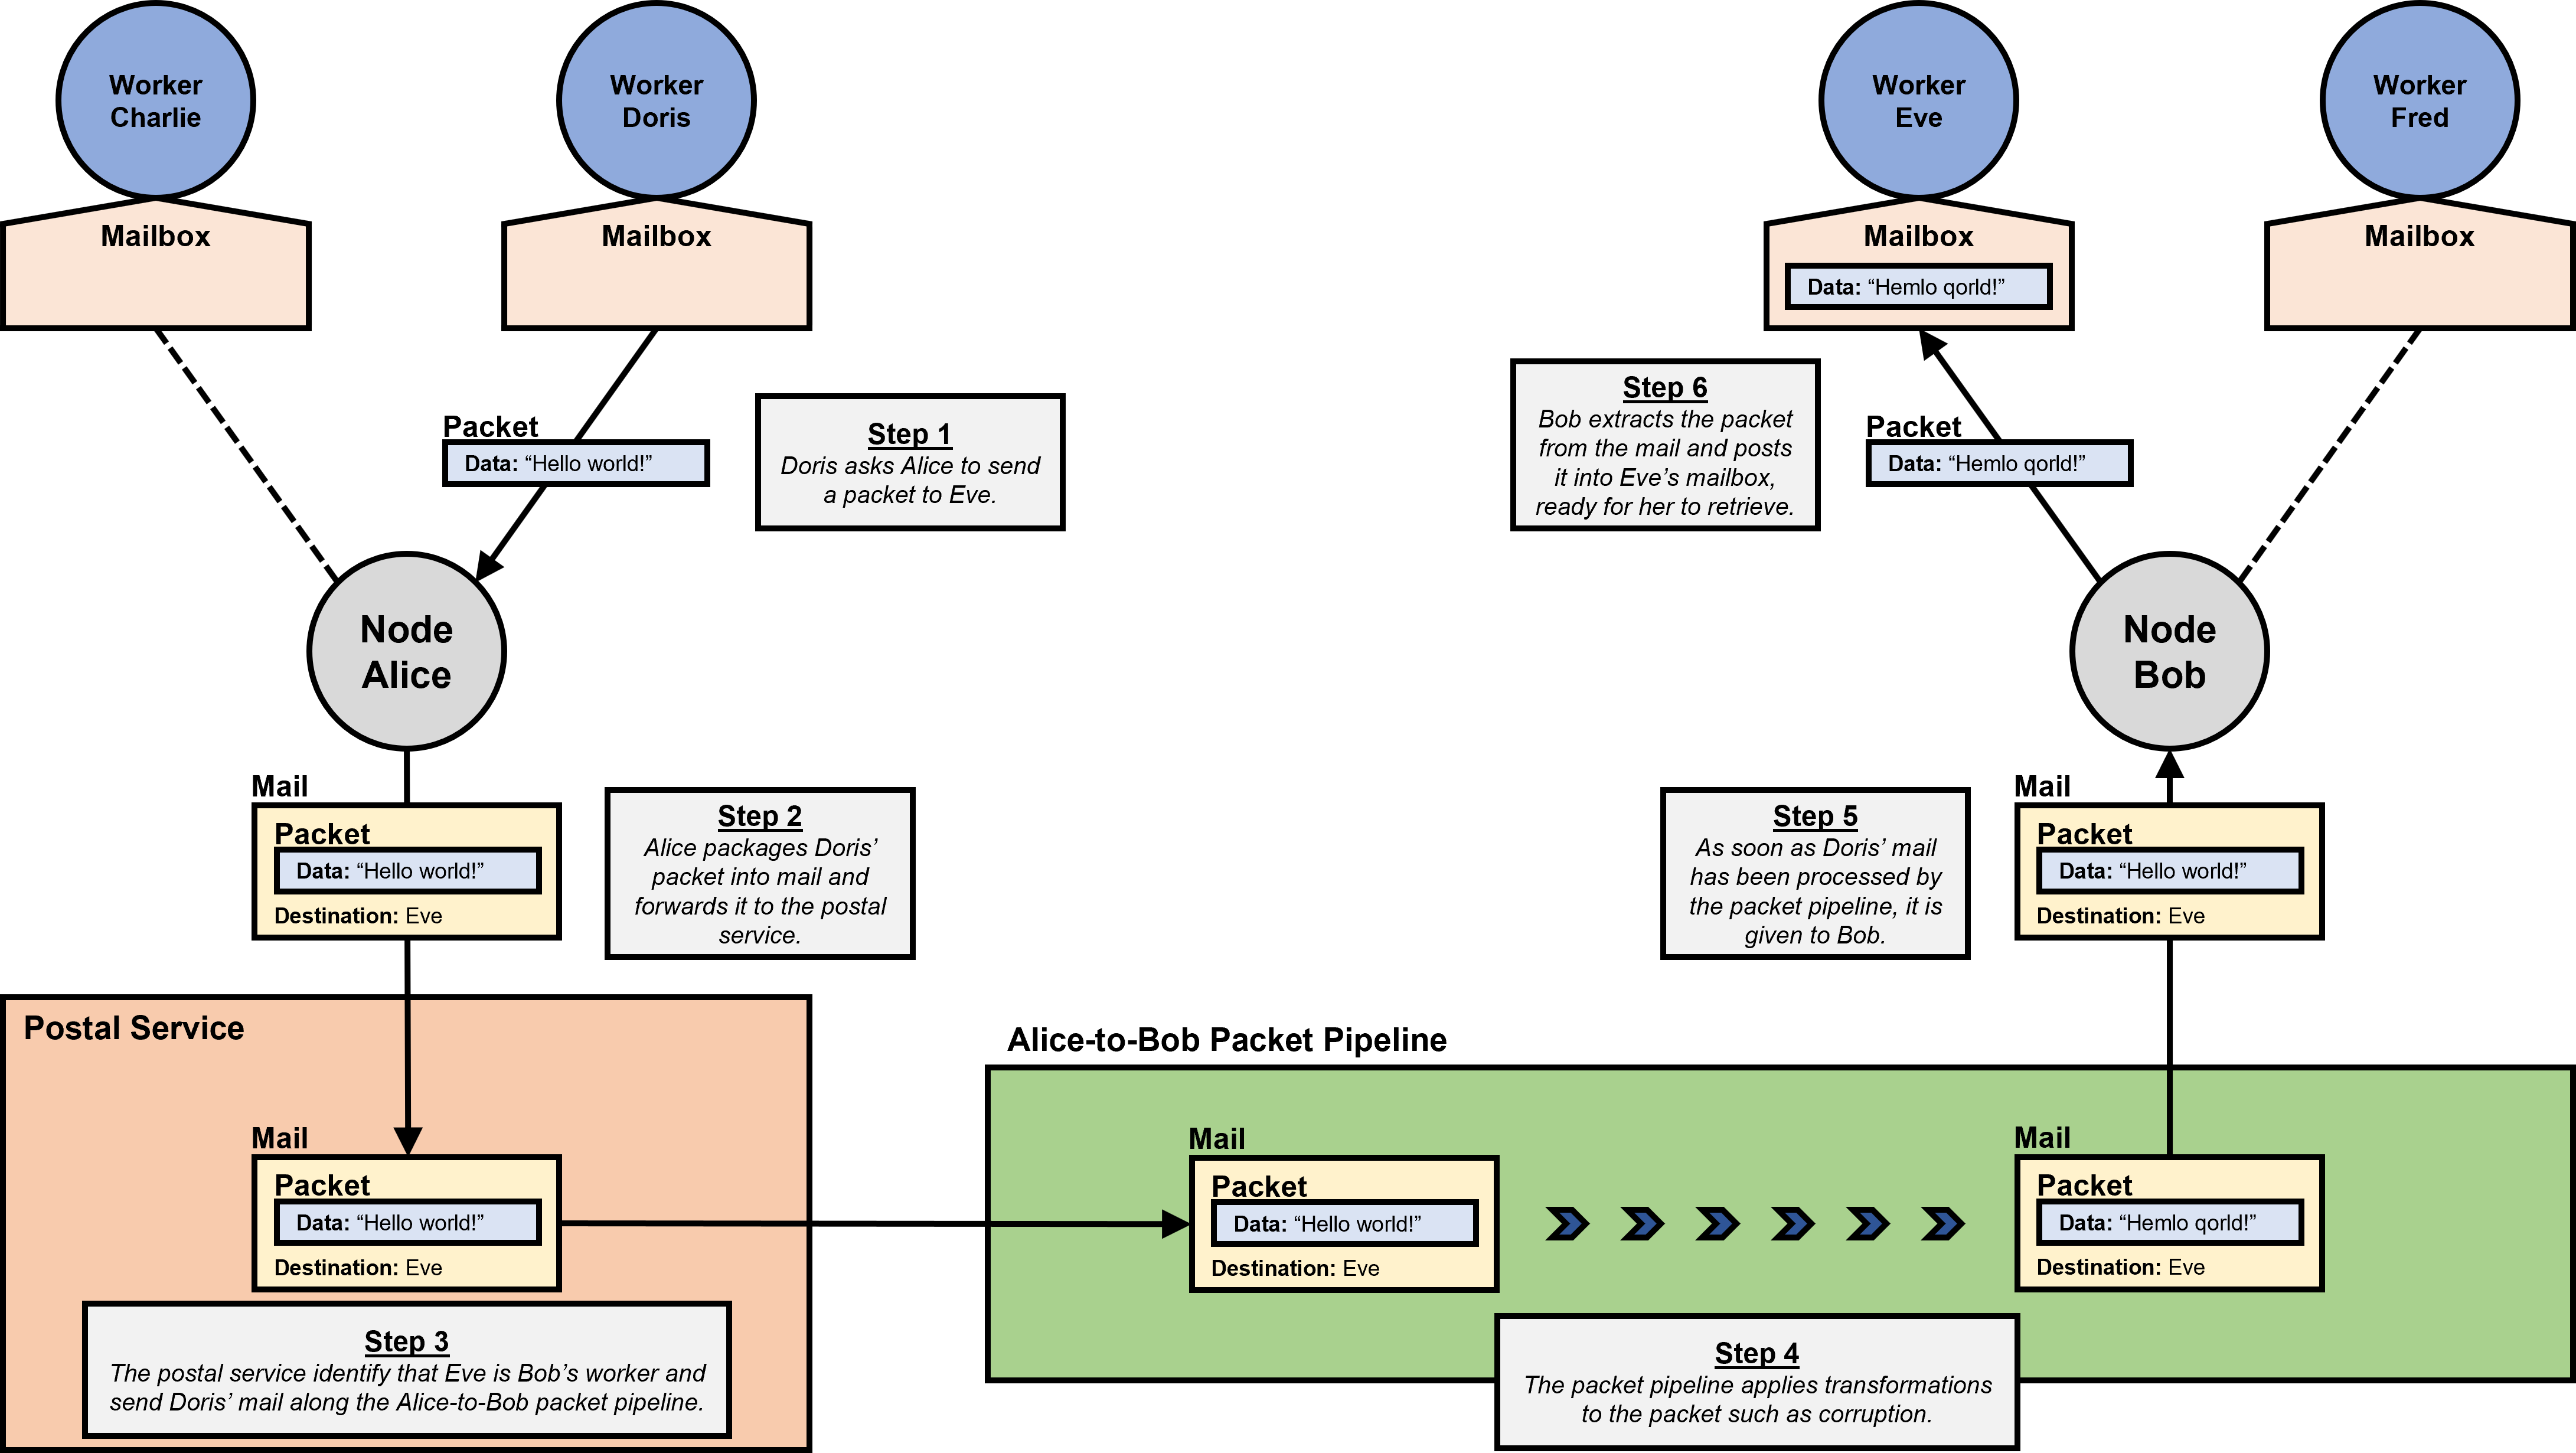
\includegraphics[width=\textwidth]{images/chapter_3_design/simulation_semantics_diagram}
    \centering
    \caption{An example of how a packet would be sent from one worker to another in a Packet Courier simulation
    .}\label{fig:chapter_3_design-simulation_semantics_diagram}
\end{figure}

In this way, workers doing work on a node can be interpreted as a group of machines being connected to a central
router. Machines can connect and disconnect freely to a router, just as workers can be spawned and killed atop a node. A
router provides each of its machines with a unique local ip-address, but has its own ip-address which it shares with
the world, just as is the case with worker and node addresses. Routers are only directly connected to their
neighbours (by definition), and as such, if a device wishes to send a message to a destination that is more than one
degree removed, then it will need to ask intermediate routers to forward the message onward. Once again, Packet
Courier is no different: nodes can only directly send mail to their immediate neighbours.

\newpage

\subsection{Network Condition Semantics}

\lettrine{W}{hen} it comes to the \emph{network} aspect of the network simulation framework that Packet Courier offers,
\texttt{tc-netem}\cite{tc_netem_wiki, tc_netem_8_man,tc_netem_src} provides an excellent template to draw from.
Indeed, Packet Courier incorporates most of the semantics that \texttt{tc-netem} lays out for itself, just with a few
subtle tweaks, namely:
\begin{itemize}
    \item \textbf{Bandwidth throttling} \\
    Constrains bitrate to a specified upper limit. \\ \\
    \emph{Packet Courier achieves this effect in a very prescriptive manner by imbuing each packet with a latency
    based on the maximum throughput and the size of the packet. For example, if the bitrate was set to 4MBps and a
    1MB packet arrived, then it would be made to wait 0.25 seconds in simulation time. This effect stacks, meaning
    that if a 2MB packet then arrived in the same tick, it would be made to wait 0.75 seconds to account for the 1MB
    of data that is yet to experience its 0.25 seconds of latency. In this way, 3MB is transferred over 0.75 seconds,
        upholding a 4MBps bitrate. \\ \\
        The general premise is to control the bitrate of a connection rather than drop excess packets. Consequently,
        packet throttling does risk becoming a black hole with respect to memory, particularly in cases where a
        high-throughput connection is being heavily throttled over a long period of time. As such, packet throttling
        should mainly be used to smooth out connections that are prone to burst behaviours, rather than as a cheap
        and dirty bitrate control mechanism. This is unlikely to satisfy users on its own, however, and as such, the
        packet throttling semantics include a drop-threshold parameter which acts as a failsafe: if the number of
        bytes currently held in the packet throttler's buffer exceeds the threshold, then incoming packets will be
        dropped until the contents of the buffer fall below this threshold again.}
    \item \textbf{Packet limiting} \\
    Enforces that only a certain number of packets can be enqueued within a certain time-frame, dropping any that
    exceed the limit. \\ \\
    \emph{Packet Courier leverages the notion of a ``packet-budget'' to decide how many packets should be enqueued
    within a particular time-frame. With each simulation tick, the time between the current simulation time and the
    last tick is measured and multiplied with the maximum number of packets per unit time to calculate the
    packet-budget, i.e.: how many packets are allowed through over the course of the next tick.}
    \item \textbf{Packet delay} \\
    Imbues packets with an artificial latency in keeping with a chosen distribution (uniform, normal or exponential).
    \\ \\
    \emph{Delay semantics are achieved by simply sampling the provided distribution and adding that value onto the
    current simulation time to produce a scheduled ``dequeue'' time. Packets can be stored in a priority queue which
    only releases the top element if the current simulation time has passed the scheduled dequeue time. \\ \\
    The only notably difference being the replacement of the Pareto distribution with the exponential distribution.
    This can be chalked up to the exponential distribution already having been implemented for other use-cases, but
    the Pareto distribution being cut due to time constraints.}
    \item \textbf{Packet drop} \\
    Samples a Bernoulli distribution and drops the packet on success. \\ \\
    \emph{Drop semantics remain the same as \texttt{tc-netem}. Gilbert Elliott and Markov modelling were left out
    because they can be replicated as part of the more general event-based semantics. ``Loss'' has been changed to
    ``drop'' to avoid confusion with notions of corruption.}
    \item \textbf{Packet corruption} \\
    Samples a Bernoulli distribution and flips a random bit on success.\\ \\
    \emph{Corruption semantics remain the same as \texttt{tc-netem}.}
    \item \textbf{Packet duplication} \\
    Samples a Poisson distribution to decide how many duplicates the given packet should have and enqueues that
    number of copies alongside the packet itself. \\ \\
    \emph{Duplication semantics remain the same as \texttt{tc-netem} with the exception that the Bernoulli distribution
    has been generalised to a Poisson distribution. Indeed, if a packet is dropped on the success of a Bernoulli
    sample with parameter $p = 0.42$, then there will be 0.42 duplicate packets on average, as would be the case with
    a Poisson distribution parameterised by $\lambda = 0.42$.}
\end{itemize}

\newpage

\subsection{Event-Based Semantics}

\lettrine{I}{n} addition to simple Bernoulli sampling, \texttt{tc-netem} offers two different stateful methods to
model packet
loss\cite{tc_netem_8_man}:
\begin{itemize}
    \item \textbf{4-state Markov model} \\
    Parameters: \emph{transition probabilities $p13$, $p31$, $p32$, $p23$ and $p14$.} \\
    Semantics: \emph{``State 1 corresponds to good reception, State 4 to independent losses, State 3 to burst losses
    and State 2 to good reception within a burst.''} \\ \\
    This can be thought of more simply as a network boasting two attributes: \emph{reception} and \emph{activity}.
    Reception can either be \emph{good} or \emph{lossy}: if it is good, then packets are not dropped; if it is lossy,
    then packets are dropped. Activity can be either \emph{gap} or \emph{burst} which have no bearing on packet drop
    in isolation. Naturally these two attributes yeild a 4-state Markov model as illustrated in
    Figure~\ref{fig:chapter_3_design-tc_netem_4_state_marvok_diagram}. \\ \\
    \begin{figure}[!h]
        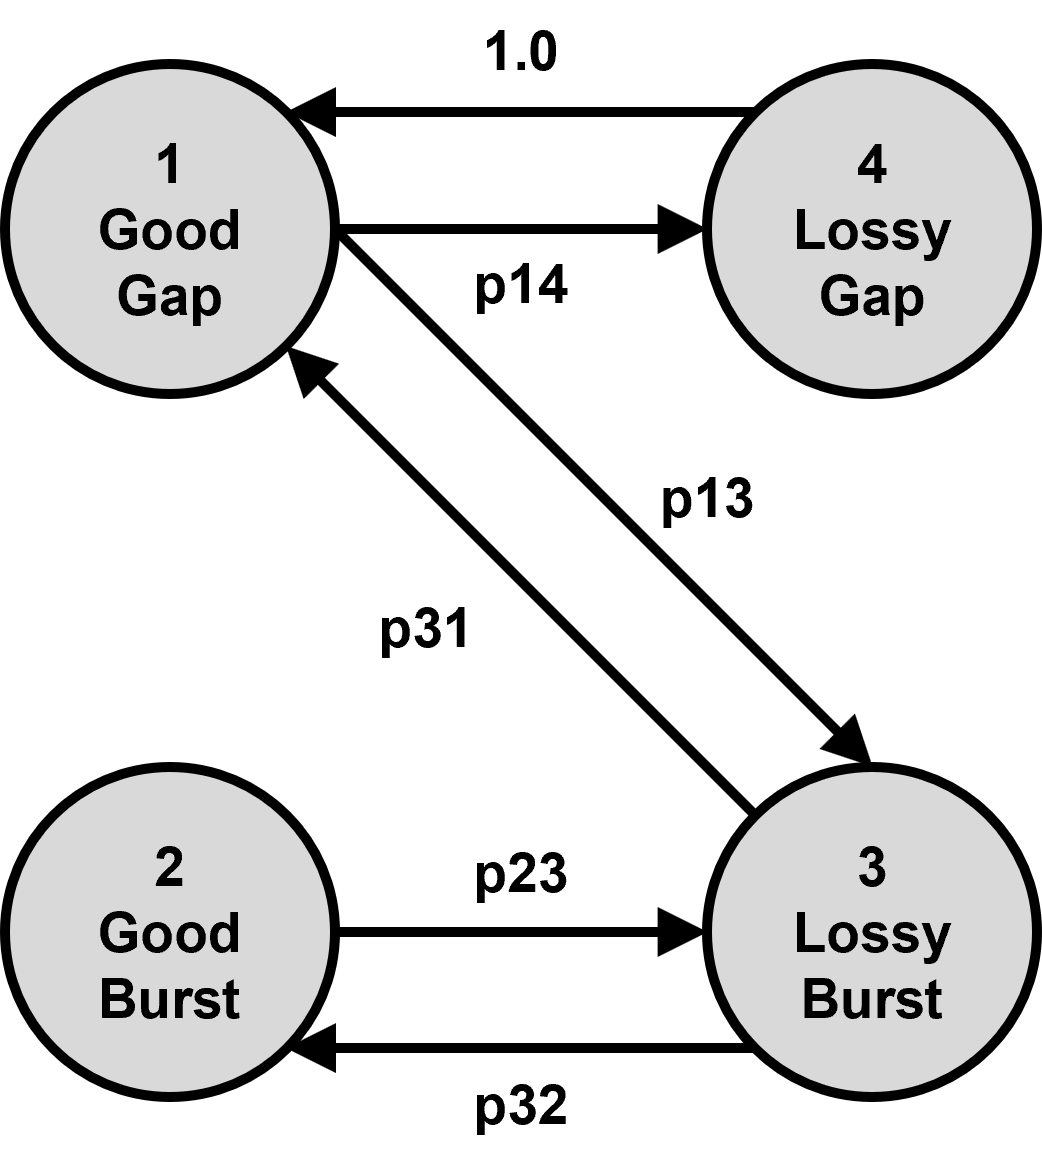
\includegraphics[width=0.35\textwidth]{images/chapter_3_design/tc_netem_4_state_marvok_diagram}
        \centering
        \caption{The 4-state Markov packet loss model as implemented by \texttt{tc-netem}\cite{tc_netem_src}
        .}\label{fig:chapter_3_design-tc_netem_4_state_marvok_diagram}
    \end{figure}

    The relevance of the activity attribute lies within the fact that the probability of a packet being dropped
    depends on which phase the network is currently undergoing: gap or burst.
    \item \textbf{Gilbert-Elliot loss model} \\
    Parameters: \emph{$p$, $r$, $h$ and $k$.} \\
    Semantics: \emph{``$p$ and $r$ are the transition probabilities between the bad and the good states, $1-h$ is the
    loss probability in the bad state and $1-k$ is the loss probability in the good state.''}
\end{itemize}

\newpage

Whilst these models do give users the opportunity to specify more complex packet drop conditions, they admit of the
following limitations:
\begin{itemize}
    \item \textbf{The 4-state Markov and Gilbert-Elliot models can only be applied to packet drop} \\
    If packet drop can be stateful, then it intuitively follows that other network artefacts can be as well. Indeed,
    one might ask: ``what causes a connection to enter into a `good burst' or a `lossy gap' phase?'' The answer will
    surely relate to underlying quirks of the network infrastructure, which are unlikely to affect loss of packets in
    a manner that is totally independent of latency, say. Even then, plenty of studies have shown (inadvertently or
    otherwise) that network phenomena such as delay and jitter can vary in ways that are seemingly
    stateful\cite{hpbn_mobile_networks, a_close_examination_of_4G_lte_networks,
        gsma_4G_5G_experience_evaluation_guideline, mobile_broadband_networks_under_mobility,
        emulating_3G_4G_networks, study_on_quality_of_service_in_4G_and_5G_networks,
        speed_test_russian_4G_LTE_internet_provider_Beeline}.
    Figure~\ref{fig:chapter_3_design-delay_plotted_against_time_from_study} shows one such example of this principle
    in action, whereby the latency observed appears to behave approximately according to a 3 state model: ``good'',
    where delay seems to mostly hover in the 25-30ms region; ``bad'', where delay will occassionally spike to as high
    as 50ms; ``ugly'', where delay very rarely spikes to even higher than 50ms. To illustrate this hypothesis
    further, we can see similar patterns when examining other metrics such as traffic load, as demonstrated in
    Figure~\ref{fig:chapter_3_design-traffic_load_plotted_against_time_from_study}. \\ \\

    \begin{figure}[!h]
        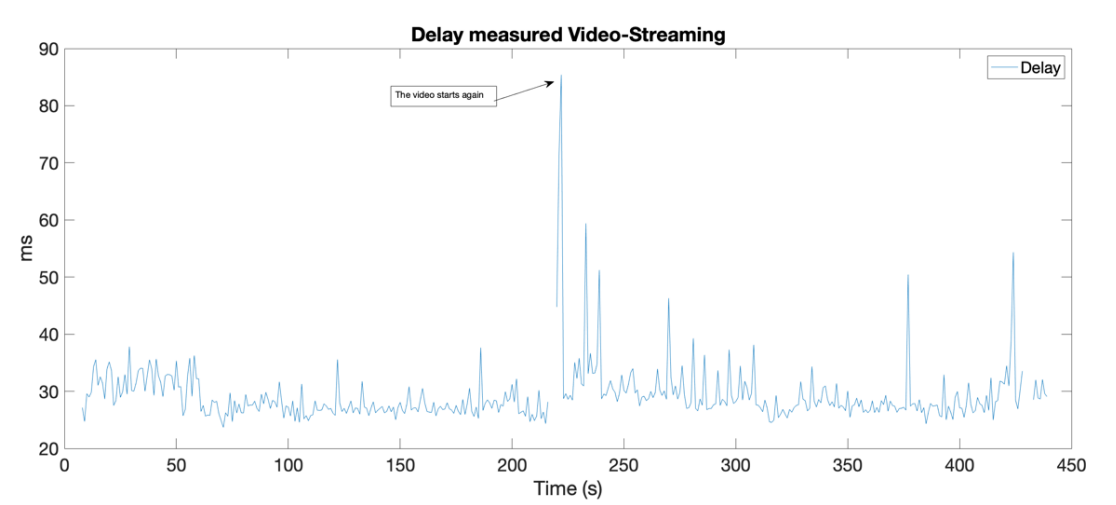
\includegraphics[width=0.9\textwidth]{images/chapter_3_design/delay_plotted_against_time_from_study}
        \centering~\caption{Delay (ms) on 4G packets bent sent as part of a video streaming service measured over
        time (s)\cite{study_on_quality_of_service_in_4G_and_5G_networks}.
        }\label{fig:chapter_3_design-delay_plotted_against_time_from_study}
    \end{figure}
    \begin{figure}[!h]
        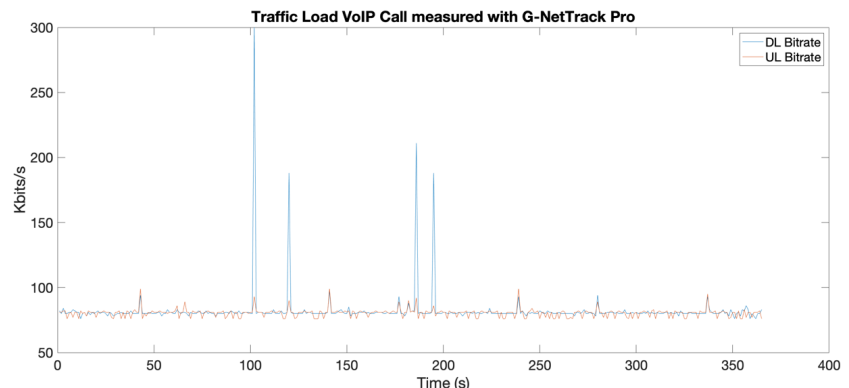
\includegraphics[width=0.9\textwidth]{images/chapter_3_design/traffic_load_plotted_against_time_from_study}
        \centering~\caption{Traffic Load (KBits/s) on 4G packets bent sent as part of a VoIP call measured over
        time (s)\cite{study_on_quality_of_service_in_4G_and_5G_networks}.
        }\label{fig:chapter_3_design-traffic_load_plotted_against_time_from_study}
    \end{figure}

    In this way, one could eyeball the number of states that would be appropriate to model the kind of conditions
    observed in Figures~\ref{fig:chapter_3_design-delay_plotted_against_time_from_study}
    and~\ref{fig:chapter_3_design-traffic_load_plotted_against_time_from_study}, only to then perform some kind of
    k-means clustering algorithm to aggregate the relevant statistics and characterise these states, i.e.: how
    frequently they occur; how long they last; how their key metric (drop, delay, traffic-load) is distributed.
    Notice that we are now in the realm of event-based semantics, where (network) events are being described by their
    interval, duration and effect, which leads nicely onto the second issue with \texttt{tc-netem}'s state-based
    models.
    \newpage
    \item \textbf{Probabilistically parameterised models are hard to reason about} \\
    Consider a network engineer who is new to a particular codebase and finds a protocol testbed with the following
    configuration:
    \begin{quote}
        \texttt{loss p13=0.5 p31=0.25 p32=0.4 p23=0.7 p14=0.15}
    \end{quote}
    There is a distinct likelihood that bafflement would ensue. \\ \\
    Although probabilistic state-based modelling can be very powerful, expressing a virtual network scenario in terms
    of state-transition probabilities does not always lend itself well to being human-readable. Most would find it
    difficult to develop a sense of how the network defined above would behave in even a coarse sense. For example,
    if packets flowed into the simulation at a constant rate, what might the graph of throughput against time look
    like? How would it be shaped? Would there be peaks and troughs, and if so, how frequently and for how long? These
    are important questions that are not necessarily self-evident from a selection of transition probabilities.
    \item \textbf{What if 4-state Markov and Gilbert-Elliot models don't fit the bill?} \\
    Unless a particular network admits of exactly one state, a ``good`` and a ``bad'' state, or four states
    characterised by ``good''/``lossy'' and ``gap''/``burst'', then it'll be a hard task to accurately model it
    using \texttt{tc-netem}. Packet loss on mobile connections has been shown to differ signicantly based on locality
    and speed of travel\cite{mobile_broadband_networks_under_mobility}, and with the gaming industry trending towards
    mobile ventures\cite{statista_mobile_gaming, rise_of_mobile_gaming}, there is a strong chance that game development
    firms will want to optimize their net-code by emulating the kind of network conditions experienced when on a
    train, bus or car journey. As such, a more general purpose set of semantics are required for undertakings of this
    nature.
\end{itemize}

\subsection{Algorithms}

\subsubsection{Normal Distribution Sampler}

TODO

\subsubsection{Poisson Distribution Sampler}

TODO


\section{Top-Down Specification}

TODO

\subsection{Application-Programmer Interface}

TODO

\subsection{Standalone Emulator}

TODO
